% ----------------------------------------------------------
% revisão bibliográfica
% ----------------------------------------------------------
\chapter[Revisão Bibliográfica]{Revisão Bibliográfica}

Este capítulo apresenta um levantamento bibliográfico sobre segurança da informação e vulnerabilidades. Tem como objetivo definir conceitos e apresentar exemplos da utilização dos termos e seus exemplos no mundo real.

% --------------------------%
% --- Conceitos Básicos --- %
\section{Segurança da Informação}

Segurança da Informação é o conjunto de orientações, normas, procedimentos, políticas e demais ações que têm por objetivo proteger o recurso informação, possibilitando que o negócio da organização seja realizado e a sua missão seja alcançada
\cite{Fontes2017}.

Proteger a informação é responsabilidade de cada pessoa na organização em que coopera e cabe à organização orientar seus colaboradores em relação à proteção da informação. De acordo com \citeonline{Spanceski2004}, uma da formas de proteger a informação é conhecer os seguintes pilares da área da segurança da informação:

\begin{itemize}
\item Autenticidade: assegura que as informações vieram da fonte anunciada;
\item Confidencialidade: protege as informações contra leituras ou cópias por pessoas não autorizadas;
\item Integridade: garante que as informações não sofram alterações indevidas sem a permissão dos proprietários das informações;
\item Disponibilidade: assegura que as informações estejam acessíveis e utilizáveis aos usuários sempre que necessários.
\end{itemize}

A importância da segurança cresce ainda mais quando os dados da organização são expostos não somente para os colaboradores mas para os usuários ou clientes finais. A falta de um planejamento em segurança pode acarretar problemas em cada um dos pilares descritos acima. Por exemplo, se um banco de dados de senhas não foi devidamente protegido contra leitura por pessoas não autorizadas, um eventual vazamento do mesmo pode representar um grande risco à confidencialidade dos envolvidos. 

\section{Vulnerabilidades}

No contexto da segurança de computadores, uma vulnerabilidade pode ser definida como uma falha em um sistema que permite a realização e a concretização de um ataque em um sistema computacional \cite{Aparecido2014}. Para explorar uma vulnerabilidade, um atacante deve ter pelo menos uma ferramenta ou técnica aplicável que possa conectar a uma fraqueza do sistema, essas ferramentas são chamadas de \textit{exploits} \cite{Whitman2011}. 

De maneira geral, vulnerabilidades possuem um ciclo de vida conforme a Figura \ref{fig:xiao}, onde a partir da descoberta de vulnerabilidades há uma corrida entre desenvolvedores/usuários e atacantes. Enquanto os desenvolvedores tentam liberar atualizações (\textit{patches}) para que os usuários possam instalar e não estarem mais vulneráveis, os atacantes tentam explorar essas vulnerabilidades por meio de ferramentas automatizadas antes que os usuários instalem as correções. 

\begin{figure}[H]
\centering
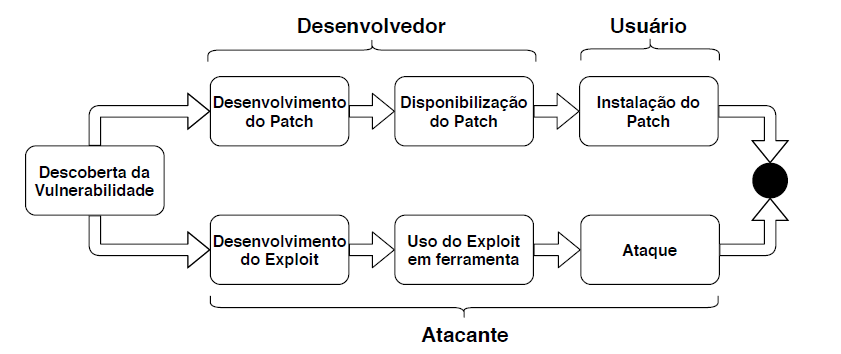
\includegraphics[width=1\textwidth]{imagens/figura_xiao.PNG}
\caption{Ciclo de vida de uma vulnerabilidade \cite{xiao2018patching}}
\label{fig:xiao}
\end{figure}

Durante a fase de descoberta de vulnerabilidades, quando desenvolvedores ou atacantes descobrem falhas no sistemas, essas vulnerabilidades podem ser divulgadas ao público. Essa divulgação pode ocorrer ou em fóruns públicos ou através da liberação de uma atualização para a correção da vulnerabilidade.

Dados sobre vulnerabilidades de segurança em software geralmente são encontradas usando portais de busca especializados em armazenar e manter informações sobre vulnerabilidades e falhas de segurança, tais como as organizações NVD \cite{NVD}, Secunia \cite{Secunia2009}, US-CERT \cite{CERT1991} e \textit{Open Source Vulnerability Database} \cite{OSVDB2002}. Para este trabalho, assim como para a maioria dos estudos acadêmicos sobre o assunto, a coleta dos dados é feita com o auxílio do portal de busca NVD.

O NVD é uma referência na coleta de dados sobre vulnerabilidade e é sincronizado com o CVE \textit{(Common Vulnerabilities and Exposures)} \cite{CVE1985}. Enquanto o CVE cadastra vulnerabilidades, o NVD categoriza e avalia os riscos delas. 

O CVE é um  banco de dados público em que todos os interessados podem obter acesso a informações sobre vulnerabilidades. O principal gestor do CVE é o MITRE \textit{(Massachusetts Institute of Technology's Digital Computer Laboratory)} e sua proposta não é somente divulgar informações sobre vulnerabilidades de segurança, e sim padronizar essas informações, com a ajuda do NVD \cite{Peotta2006}. 

Um exemplo de vulnerabilidade reportada pelo NVD é mostrada na Figura \ref{fig:nvd1}. A plataforma do NVD disponibiliza todos os CVEs existentes desde 1988 até o ano atual. Para cada ano é possível escolher um mês e visualizar todas as vulnerabilidades divulgadas naquele período, mas não são todos os anos que tem os doze meses divulgados. Foi escolhido para esse exemplo o mês de abril do ano de 2012. 

\begin{figure}[H]
\centering
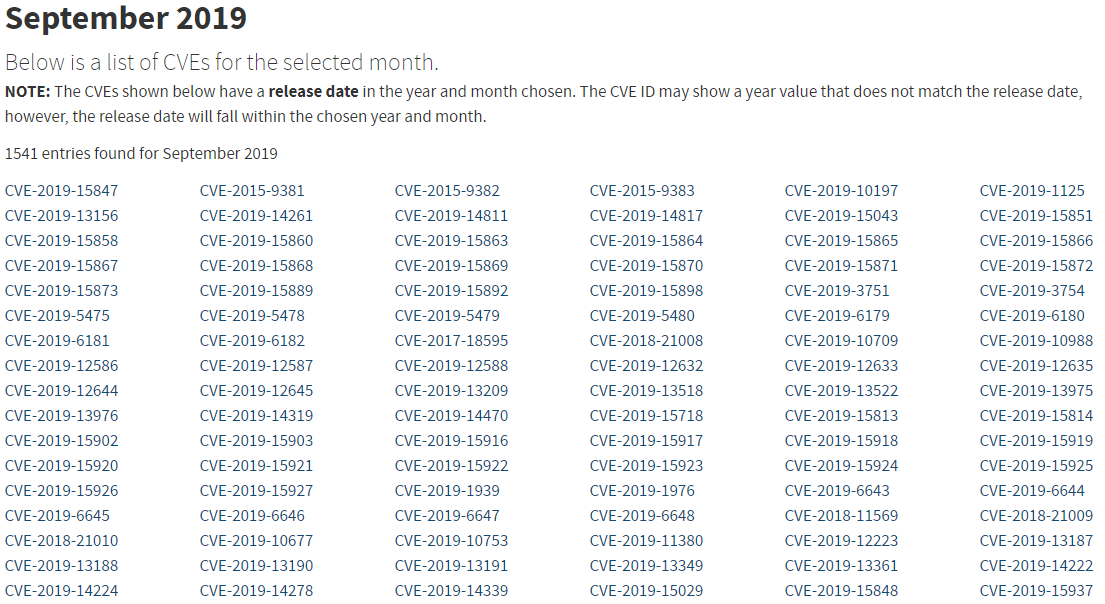
\includegraphics[width=1\textwidth]{imagens/nvd_exemplo1.png}
\caption{Vulnerabilidades reportadas pelo NVD em abril de 2012}
\label{fig:nvd1}
\end{figure}

A Figura \ref{fig:nvd1} mostra parte das 228 vulnerabilidades divulgadas para o ano de 2012 no mês de abril. Ao selecionar qualquer CVE, uma nova página é carregada com os detalhes da vulnerabilidade escolhida. Para este exemplo, o primeiro CVE-2011-4042 é apresentado na Figura \ref{fig:nvd3}.

\begin{figure}[H]
\centering
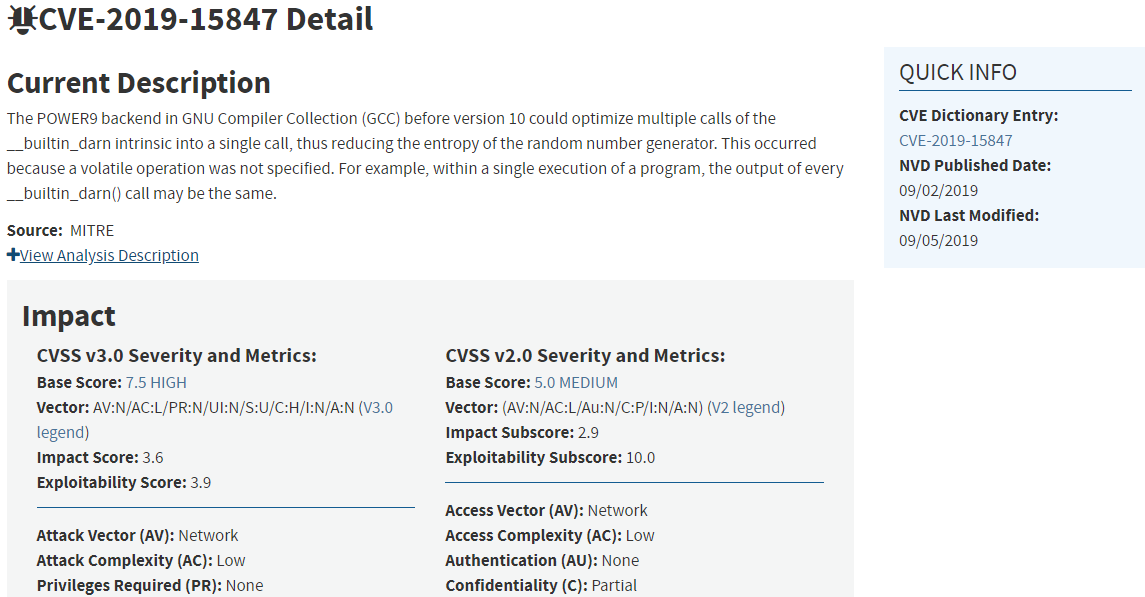
\includegraphics[width=1\textwidth]{imagens/nvd_exemplo3.png}
\caption{Vulnerabilidade CVE-2011-4042}
\label{fig:nvd3}
\end{figure}

A Figura \ref{fig:nvd3} mostra alguns detalhes relacionados a vulnerabilidade CVE-2011-4042.  Descrição \textit{(Description na Figura)}, a tabela de impacto \textit{(Impact na Figura)} e a data de publicação da vulnerabilidade \textit{(NVD Published Date na Figura)}, são alguns dos campos apresentados em arquivos XML sendo identificados no cabeçalho principal do arquivo. Esse cabeçalho serve para facilitar na busca dos dados para a coleta.

% -------------------------------%
% --- Trabalhos Relacionados --- %
\section{Trabalhos Relacionados}

Esta seção tem como objetivo descrever trabalhos relacionados ao tema principal desse trabalho: análise de descoberta de vulnerabilidade. Os trabalhos propostos por \citeonline{Massacci2014}, \citeonline{Alhazmi2007}, \citeonline{Alhazmi2008} e \citeonline{Joh2016} serão apresentados a seguir. Ao final, será discutido brevemente a relação destes trabalhos com a proposta deste trabalho.

Um modelo de descoberta de vulnerabilidade pode ser usado para avaliar e prever tendências futuras acerca de descoberta de vulnerabilidade de software. Ou seja, os modelos usam dados antigos de vulnerabilidades divulgadas (em geral fornecidos por bases de dados que catalogam vulnerabilidades de segurança, como a NVD) para tentar prever a ocorrência de novas vulnerabilidades no futuro.

Dentre os diversos modelos estatísticos usados para analisar as características do processo de descoberta de vulnerabilidade, têm-se:

\begin{itemize}
\item Modelo Logístico Alhazmi-Malaiya (AML) e Modelo Linear (LN) proposto por Alhazmi e Malaiya \cite{Alhazmi2006};
\item Modelo Quadrático (RQ) e Modelo Exponencial (RE) proposto por \cite{Rescorla2005};
\item Modelo Weibull (JW) proposto por Kim et al. \cite{Joh2008a};
\item Modelo Distribuição Normal Dobrada (YF) proposto por Younis et al. \cite{Younis2011};
\item Modelo Termodinâmico (AT) proposto por \cite{Anderson2002};
\item Modelo Regressão de Poisson (LP) proposto por Musa e Okumoto \cite{Musa:1984:LPE:800054.801975}.
\end{itemize}

Alguns modelos de crescimento de confiabilidade de software (RGB) também usam VDMs para estudar o processo de detecção de defeitos \cite{Ozment2006}, \cite{Musa2004} em sistemas computacionais.

\citeonline{Massacci2014} apresentam uma metodologia empírica que avalia sistematicamente o desempenho de VDMs em duas dimensões (qualidade e previsibilidade) e abordam todas as questões identificadas da metodologia tradicional, isto é, questões que distorciam estudos prévios no campo. 

Para ilustrar a metodologia, os autores fizeram um experimento para avaliar oito VDMs (AML, AT, LN, JW, LP, RE, RQ e YF) em 30 lançamentos principais de quatro navegadores da Web: IE, Firefox, Chrome e Safari. Classificaram a idade da versão de um navegador em três períodos diferentes: juventude (dentro de 6 - 12 meses desde a data de lançamento), idade média (12 a 36 meses desde a data de liberação) e idade avançada (36 meses). 

Os autores descobriram que se uma versão é relativamente nova, então o melhor modelo a ser usado é um modelo linear para estimar as vulnerabilidades nos próximos 3 - 6 meses. Para navegadores de meia-idade e idade avançada, o melhor é usar um modelo logístico em forma de "s". Em comparação com a metodologia tradicional, isso teria sido impossível.

\citeonline{Alhazmi2007} investigam em seu artigo se é possível prever o número de vulnerabilidades que podem estar potencialmente presentes em um sistema de software, mas que ainda não foram encontradas. Os autores usaram vários sistemas operacionais como representantes de sistemas de software complexos, tais como Windows 95, Windows 98, Windows XP, Windows NT4, Windows 2000, Windows 2003, Red Hat 6.2 e Red Hat 7.1.

Além dos dados sobre vulnerabilidades descobertas nesses sistemas, os autores examinaram os resultados para determinar se a densidade de vulnerabilidades em um programa é uma medida útil tanto para os usuários quanto para os desenvolvedores. A densidade de vulnerabilidades pode ser usada pelos usuários para avaliar o risco ao considerar a compra de um novo sistema de software da mesma empresa e os desenvolvedores podem usar essa métrica para estimar quantidades de vulnerabilidades que provavelmente serão descobertas dentro de algum período de tempo futuro para decidir se adia a aplicação de patches examinando os riscos de modo a evitar a desestabilização dos sistemas de software.

Por fim, os autores consideraram a taxa de descoberta de vulnerabilidades para verificar se os modelos de descoberta de vulnerabilidades podem ser desenvolvidos para projetar tendências futuras. Os resultados revelaram que é possível modelar a descoberta de vulnerabilidades usando um modelo logístico (AML) que às vezes pode ser aproximado por um modelo linear.

\citeonline{Alhazmi2008} descrevem a aplicabilidade e a significância dos parâmetros de seis modelos de descoberta de vulnerabilidade (AT, AML, LM, LP, RQ, RE) para quatro sistemas operacionais (Windows XP, Windows 95, Red Hat Linux 6.2 e Red Hat Fedora). Os modelos de descoberta de vulnerabilidade foram examinados usando o critério de informação de Akaike (AIC) e teste qui-quadrado. A avaliação descobriu que o modelo AML é geralmente melhor a longo prazo, com melhor desempenho para sistemas como o Windows 95, Red Hat Linux 6.2 e Red Hat Fedora. 

Além do trabalho publicado em 2009, os autores Joh e Malayia publicaram um outro trabalho, com uma metodologia semelhante, em 2016 \cite{Joh2016}. Este último trabalho condensa os dados entre 1995 e 2015. Os autores examinaram vulnerabilidades divulgadas em diversos softwares (Sistemas operacionais Windows: Windows NT, Windows 95, Windows 98, Windows 2000, Windows XP e Windows 7; Sistemas operacionais diferentes do Windows: iOS, MAC OS X, Red Hat Linux Enterprise, AIX, Android e Chrome OS; e outros sistemas: Apache, IIS, Internet Explorer, Firefox, Safari e Java (JRE)) para investigar possíveis variações anuais nos processos de descoberta de vulnerabilidades. Também examinaram a periodicidade semanal na distribuição de atualizações de segurança (patches) e exploração das vulnerabilidades. 

Para todos os grupos de software examinados pelos autores, uma taxa de descoberta de vulnerabilidades mais alta é encontrada em determinados meses. Nos produtos Microsoft, uma incidência mais alta durante os períodos de meio ano é observada. Além disso, o comportamento periódico de 7 dias foi observado nos dados de varredura de vulnerabilidades; maior atividade durante a semana  do que nos fins de semana foi confirmada. Especificamente, os valores da atividade de vulnerabilidade correspondentes a terça-feira tenderam a ser maiores do que os outros dias da semana. Os resultados mostraram que a periodicidade precisa ser considerada para a alocação ótima de recursos e para a avaliação dos riscos de segurança.

Apesar dos trabalhos \citeonline{Massacci2014}, \citeonline{Alhazmi2006}, \citeonline{Alhazmi2008}, \citeonline{Joh2009} e \citeonline{Joh2016} conduzirem estudos para modelar o processo de descoberta de vulnerabilidade de software, somente os dois últimos detalham a questão da sazonalidade. O objetivo do presente trabalho é comparar os resultados da análise da sazonalidade em dois diferentes momentos: entre 1995-2007 e entre 2008-2017. A principal motivação para isso é avaliar a evolução do comportamento de questões de segurança ao longo dos anos.